\documentclass[8pt,a4paper,landscape]{extarticle}
% -- Layout ----
\usepackage[top=0.6cm, bottom=0.6cm, left=0.5cm, right=0.5cm, landscape]{geometry}

% -- Titles ----
\usepackage[
  tiny,                     % text size title
  compact                   % reduce vertical space before/after title
]{titlesec}
% \titlespacing*
\titleformat{\section}{\normalfont\small\bfseries}{\thesection}{0em}{} % Remove space before and after section titles
\titleformat{\subsection}{\normalfont\small\bfseries}{\thesubsection}{0em}{} % Remove space before and after subsection titles
\titlespacing*{\section}{0pt}{0pt}{0pt} % Remove space before/after section titles
\titlespacing*{\subsection}{0pt}{0pt}{0pt} % Remove space before/after subsec titles

% -- Colors ----
\usepackage[dvipsnames]{xcolor}
\definecolor{dmm}{RGB}{192,192,192} % Define a custom dimmed text color
\definecolor{cmt}{RGB}{61,123,123}

% -- Math ------
\usepackage{mathtools}
\usepackage{amssymb}
\usepackage{turnstile}%better vdash

% -- Lists -----
\usepackage[inline]{enumitem}
\setlist{noitemsep}% Remove vspace between items
% Set vspace before and after  list environments as well as the left margin
\setlist[itemize,1]{leftmargin=.6em,labelindent=0pt,labelsep=2pt,
  topsep=1pt,partopsep=1pt}
\setlist[enumerate,1]{leftmargin=1em,labelindent=0pt,labelsep=2pt,
  topsep=1pt,partopsep=1pt}
\setlist[itemize,2]{leftmargin=.3em,labelindent=1pt,topsep=1pt,partopsep=1pt}
\setlist[enumerate,2]{leftmargin=0.2em,labelindent=1pt,topsep=1pt,partopsep=1pt}
\setlist[description]{labelwidth=\linewidth,font=\small\bfseries,leftmargin=1em,topsep=1pt,partopsep=1pt}
% -- Code listing ---
\usepackage{listings}
\lstset{
  aboveskip=3pt,
  belowskip=3pt,
  basicstyle=\small\ttfamily,
  breaklines=true,
  % commentstyle=\upshape\ttfamily,
  captionpos=b,
  commentstyle=\color{cmt},
  frame=single,
  keepspaces=false,
  keywordstyle=\bfseries,
  showspaces=false,
  showstringspaces=false,
  showtabs=false,
  tabsize=2,
}

% Parse Trees
\usepackage{tikz}
\usetikzlibrary{ arrows, automata, bbox, calc, positioning,  decorations.pathmorphing, decorations.pathreplacing, decorations.shapes, }
\tikzset{
% ->, % makes the edges directed
>=stealth', % makes the arrow heads bold
node distance=1cm, % specifies minimum distance between two nodes
% small/.style={},
every state/.style={thick}, % sets the properties for each ’state’ node
every node/.style={inner sep=1pt},
initial text=start, % sets the text that appears on the start arrow
}

% Place a figure env right here via [H] option
\usepackage{float}

% Side by side figure
\usepackage{subcaption}
% \usepackage{caption}
% \captionsetup{belowskip=0pt, aboveskip=0pt}


% -- Multi-Col layout --
\usepackage{multicol}

% No indentation
\setlength\parindent{0pt}
\setlength\abovedisplayskip{-5pt}
\setlength\belowdisplayskip{-5pt}
\setlength\abovedisplayshortskip{-4pt}
\setlength\belowdisplayshortskip{-4pt}
\newcommand{\gor}{\;|\;}
\newcommand{\num}{\texttt{\#}~}
\renewcommand{\arraystretch}{1.2}


\begin{document}
% Suppress page number for all pages
\pagestyle{empty}

% Notes begin
\begin{multicols*}{3}
% \section*{Memory (compiled and runnable \texttt{!=} correct)}
\begin{tabular}[th!]{l|ccc}
  \hline
  type & allocation & deallocation & life cycle \\
  \hline
  stack* & implicit (compiler) & implicit (compiler) & short \\
  heap & explicit (user) & explicit (user) & long \\
  \hline
  \multicolumn{3}{l}{*: also called \textbf{automatic} memory}\\
  \hline
\end{tabular}
\begin{tabular}[th!]{l|lp{6.5cm}}
  \hline
  name & type & usage \\
  \hline
  \texttt{malloc} & lib call & dynamic memory alloc without zeroing \\
  \texttt{calloc} & lib call & dynamic memory alloc with zeroing\\
  \texttt{realloc} & lib call & dynamic memory allocation \\
  \texttt{free} & lib call & only accepts memory alloced by \texttt{re/malloc} \\
  \texttt{brk} & sys call & sets program break to specific value; user programs should avoid using it directly \\
  \texttt{sbrk} & sys call & increment program break by n bytes; user programs should avoid using it directly \\
  \texttt{mmap} & sys call & commonly used by allocator, not by user programs \\
  \hline
\end{tabular}
\begin{itemize}
\item idiom for string: \texttt{malloc(strlen(s) + 1)}
\item the size of allocated region \emph{must} be tracked by memory-allocator itself
\end{itemize}
\section*{Common memory errors}
\begin{enumerate}
\item Forget to Allocate Memory
  \begin{lstlisting}[language=c,xrightmargin=2pt]
char *src = "hello";
char *dst; // oops! unallocated; (char *) malloc(5 * sizeof char)
strcpy(dst, src); // segfault
\end{lstlisting}

\item Not Allocate Enough Memory (buffer overflow)
\begin{lstlisting}[language=c,xrightmargin=2pt]
char *src = "hello";
char *dst = (char *) malloc(strlen(src)); // too small!
strcpy(dst, src); // may work properly
\end{lstlisting}

\item Forget to Initialize Allocated Memory
  \begin{itemize}
  \item Will eventually encounter an uninitialized read (undefined behavior)
  \item Out-of-bound read/write
  \end{itemize}

\item Forget to Free Memory (memory leak)
  \begin{itemize}
  \item In long-running apps or systems (such as OS itself), slowly leaking memory eventually results in running out of memory
  \item For short-lived, soon-exiting programs, OS will clean up, thus \emph{no} memory leak (bad habit anyway)
  \end{itemize}

\item Use-after-free (dangling pointer)
\item Free Memory Repeatedly (double free)
\item Call \texttt{free()} Incorrectly (invalid free)
  \begin{itemize}
  \item Freeing an uninitialized/arbitrary pointer
  \item Freeing the wrong pointer or freeing NULL pointer
  \end{itemize}
\end{enumerate}
\subsection*{Two levels of memory management in system}

\begin{enumerate}
\item performed by the OS, which hands out memory to processes when they run, and takes it back when processes exit (or otherwise die)
\item \emph{within} each process, e.g. when calling \texttt{malloc()} or \texttt{free()}.  OS will reclaim \emph{all} the memory of the process (including those pages for code, stack and heap) when program is finished running. No matter what the state of your heap in your address space, the OS takes back all of those pages when the process dies, thus ensuring that no memory is lost despite the fact that you didn’t free it.
\end{enumerate}
\subsection*{Reasons for dynamic memory}
\begin{itemize}
\item the amount of required memory may be task dependent
\item input size may be unknown at compile time
\item conservative pre-allocation would be wasteful
\item recursive functions
\end{itemize}

% \section*{Goals of Virtual Memory (VM) system}
\begin{enumerate}
\item \textbf{transparency} invisible to running prog (illusion: private ph. mem)
\item \textbf{efficiency} OS needs hardware support (e.g. TLBs)
  \begin{itemize}
  \item time (not making programs run much more slowly)
  \item space (not using too much mem for structs to support virtualization)
  \end{itemize}
\item \textbf{protection} thus enables isolation among processes
\end{enumerate}
\section*{Address Translation (hardware-based)}
\begin{minipage}{\linewidth}
  \centering
  \texttt{physical address = virtual address + base}
\end{minipage}
\begin{minipage}{0.45\linewidth}
  \begin{enumerate}
  \item Each memory reference by a process is a virtual address
  \item isolation property is satisfied (security)
  \item translation and check are cheap (performance)
  \end{enumerate}
\end{minipage}
\begin{minipage}{.5\linewidth}
  \begin{lstlisting}[language=c,xleftmargin=2pt]
if (addr < bounds)
  return *(base + addr);
else
  throw new SegFaultException;
// Waste physical mem (must alloc all)
// No (easy) sharing btw procs
\end{lstlisting}
\end{minipage}

\section*{Dynamic Relocation: Hardware Requirements}
\begin{tabular}[th!]{p{3.5cm}p{5.4cm}}
  Hardware Requirements & Notes \\
  \hline
  Privileged mode & Needed to prevent user-mode processes from executing privileged operations \\
  \hline
  Base/bounds registers & Need pair of registers per CPU to support address translation and bounds checks \\
  \hline
  Able to translate virtual addr and check bounds & Circuitry to do translations and check limits; in this case, quite simple\\
  \hline
  Privileged instructions to update base/bounds & OS must be ablt to set these values before letting a user program run \\
  \hline
  Privileged instructions to register exception handlers & OS must be able to tell hardware what code to run if exception occurs \\
  \hline
  Able to raise exceptions & When processes try to access privileged instructions or out-of-bounds memory \\
  \hline
\end{tabular}
\section*{Hardware support in base/bounds virtual memory}
\begin{enumerate}
\item provide 2 different CPU modes
  \begin{itemize}
  \item privileged mode (kernel mode) to access entire machine
  \item user mode (limited direction execution)
  \item a single bit stored in processor status word indicating current mode
  \end{itemize}
\item provide base and bounds registers (MMU)
\item provide \textbf{privileged} instructions to modify the base/bounds registers
\item provide exception handler to handle exceptions generated by CPU
  \begin{itemize}
  \item CPU should stop executing user program and raise exception
  \item CPU should be able to inform OS of handlers location (privileged)
  \end{itemize}
\end{enumerate}
\section*{Dynamic Relocation: Hardware Requirements}
\begin{tabular}[th!]{p{3cm}p{6cm}}
  OS Requirements & Notes \\
  \hline
  Memory management & \parbox[t]{6cm}{Need to allocate memory for new processes\\
  Reclaim memory from terminated processes \\
  Generally manage memory via \textbf{free list}} \\
  \hline
  Base/bounds management & Must set base/bounds properly on context switch\\
  \hline
  Exception handling  & \parbox[t]{6cm}{Code to run when exception arise\\
  liley action is to terminate offending process} \\
  \hline
\end{tabular}
\section*{OS support in base/bounds virtual memory}
\begin{enumerate}
\item when a process is created, finding space for its addr space in memory
\item when a process is terminated (exits gracefully or forcefully killed), reclaiming all of its memory (putting back to free list).
\item when a context switch occurs, performing a few additional steps: save and restore base-and-bounds pair to memory in process structure or process control block (PCB)
\item must provide exception handlers
\end{enumerate}

% \section*{Segmentation: Generalized Base/bounds}
\begin{minipage}{.6\linewidth}
  \includegraphics[width=\linewidth]{imgs/addr_map}
\end{minipage}
\begin{minipage}{.4\linewidth}
  \begin{tabular}[th!]{lccl}
    Seg. & Base & Size & Offset\\
    \hline
    Code & 32K  & 2K   & 0     \\
    Heap & 34K  & 3K   & 4K    \\
    Stak & 28K  & 2K   & 16K*   \\
    \hline
    \multicolumn{4}{l}{* stack grows to lower addr} \\
    \hline
  \end{tabular}
  Given addr in the segment:\\
  new = addr \textcolor{err}{-} offset + base
  \begin{itemize}
  \item Addr 100 in code segment:
  \item[] 100 - 0 + 32K = 32868
  \item Addr 4200 in heap segment:
  \item[] 4200 - 4K + 32K = 34920
  \item Addr 7100 $\to$ seg. fault
  \end{itemize}
\end{minipage}
\section*{Segment Reference (explicit approach)}
\includegraphics[width=\linewidth]{imgs/explicit2}
\begin{itemize}
\item one segment is unused $\to$ put code in heap to use 1 bit for segment
\item virtual address space is limited to 4KB (max in this example)
\end{itemize}
\section*{Stack and Sharing}
\begin{tabular}[th!]{lcclll}
  Seg. & Base & Size (max 4K) & Offset & Grows pos? & Protection*\\
  \hline
  Code$_{00}$ & 32K  & 2K   & 0    & 1 & Read-Exec  \\
  Heap$_{01}$ & 34K  & 3K   & 4K   & 1 & Read-Write \\
  Stak$_{11}$ & 28K  & 2K   & 16K  & 0 & Read-Write \\
  \hline
  \multicolumn{6}{l}{* protection bits in hardware is to support code sharing} \\
  \hline
\end{tabular}
Virtual addr: 11 1100 0000 0000 $\to$ 15K (0x3c00)
\begin{itemize}
\item 11 $\to$ in stack segment and left 3K (1100 0000 0000)
\item mapped = 3K - 4K (max segment size) + 28K (base) = 27K
\end{itemize}

% \section*{Arithmetics in Paging (Size, Page Numbers, PTE numbers)}
\begin{minipage}{0.55\linewidth}
  \includegraphics[width=\linewidth]{imgs/virtual_addr_eg}
  \flushleft
  \begin{itemize}
  \item $S_{\text{AS}}$ = 16KB = $16 \times 1024 = 2^{4} \times 2^{10} = 2 ^{14}$B
  \item V Addr bit width = $\log_2 S_{\text{AP}} = 14$
  \item $S_{\text{P}}$ = 64B = $2^{6}$B
  \item \textbf{Offset} bit width = $\log_2 S_{\text{P}} = 6$
  \item VPN bit width = 14 - 6 = 8
  \item $N_{\text{P}}$ = $\frac{S_{\text{AS}}}{S_{\text{P}}} = \frac{2^{14}}{2^{6}} = 2^{8}$
  \item $N_{\text{PTE}} = N_{\text{P}} = 2^{8} = 256$ (linear PT)
  \end{itemize}
\end{minipage}
\begin{minipage}{0.45\linewidth}
  \includegraphics[width=\linewidth]{imgs/pte_4byte}
  \flushleft
  \begin{itemize}
  \item $S_{\text{PTE}} =4$B
  \item $S_{\text{PT}} = N_{\text{PTE}} \times S_{\text{PTE}} = 1\text{KB} $
  \item Page table can be divided into pages (for 2-level PT)
  \item[] $S_{\text{PTP}} = \frac{S_{\text{PT}}}{S_{\text{P}}} = \frac{1024}{64} = 16$
  \item Each PDE points to a PTP of 16 PTEs
  \end{itemize}
\end{minipage}


% \pagebreak
% \section*{Paging: Two Advantages and Address Translation}
\begin{enumerate}
\item \textbf{flexibility}: support abstraction of address space: no need to assume direction of stack/heap growth and how they are used
\item \textbf{simplicity}: easy to manage free space: simply keep a list of free pages
\end{enumerate}
\includegraphics[width=\linewidth,height=4.5cm]{imgs/page_table}
\includegraphics[width=\linewidth,height=4cm]{imgs/address_trans}
\section*{Page Table Issues: too big and too slow}
\begin{minipage}{0.5\linewidth}
  \flushleft
  \begin{itemize}
  \item 32-bit addr space, 4K pages: 20-bit VPN, 12-bit offset
  \item $2^{20} \approx 1$ million entries in page table for 1 process
  \item Assume each \textbf{PTE} needs 4B, 1 proc needs 4MB page table!
  \item Too big for MMU: physical memory or disk (by swapping page frams in/out of mem to disk)
  \end{itemize}
\end{minipage}
\begin{minipage}{0.5\linewidth}
  \begin{itemize}
  \item Extract VPN from virtual addr (VA) to find PFN
  \item Locate page table (e.g. in a page-table reg.)
  \item Compute addr of PTE for VPN
  \item Extract offset from VA and compute physical addr (PA)
  \item Fetch data from memory at PA
  \end{itemize}
\end{minipage}
\section*{Page Table Entry (PTE)}
Each PTE needs to store target PFN plus a few more information:
\begin{itemize}
\item valid bit: whether the VPN is mapped or not
\item protection bits: whether page is for read/write/code-execution
\item present bit: whether page is in memory or disk (swapped out)
\item dirty bit: page modified since it's brought to memory (swapping on)
\item reference bit: page has been accessed; for policies for page replacement
\end{itemize}
\section*{Accessing Memory With Paging}
\begin{lstlisting}[language=c]
VPN = (VirtualAddr & VPN_MASK) >> SHIFT    // get VPN from VA
PTEAddr = PTBR + (VPN * sizeof(PTE))        // compute PET addr
PTE = AccessMemory(PTEAddr)                 // fetch PTE
// Check if process can access the page
if (PTE.Valid == False)
  RaiseException(SEGMENTATION_FAULT)
else if (CanAccess(PTE.ProtectBits) == False)
  RaiseException(PROTECTION_FAULT)
else
  offset = VirtualAddress & OFFSET_MASK           // access ok
  PhysAddr = (PTE.PFN << PFN_SHIFT) | offset      // form physical addr
  Register = AccessMemory(PhysAddr)               // fetch it
\end{lstlisting}

% \columnbreak
% \section*{TLB (faster translation)}
TLB performance (cache perf. in general) improved by two factors:
\begin{enumerate}
\item Spatial locality:  if a program accesses memory at address x , it
will likely soon access memory near x
\item Temporal locality:  ix recently accessed will likely be accessed soon
\end{enumerate}
\section*{TLB Control Flow Algorithm}
\begin{minipage}{.66\linewidth}
\begin{lstlisting}[language=c]
VPN = (VirtualAddr & VPN_MASK) >> SHIFT
(Success, TlbEntry) = TLB_Lookup(VPN)
if (Success == True) // TLB Hit
  if (CanAccess(TlbEntry.ProtectBits) == True)
    Offset = VirtualAddr & OFFSET_MASK
    PhysAddr = (TlbEntry.PFN << SHIFT) | Offset
    Register = AccessMemory(PhysAddr)
  else
    RaiseException(PROTECTION_FAULT)
else // TLB Miss
  PTEAddr = PTBR + (VPN * sizeof(PTE))
  PTE = AccessMemory(PTEAddr)
  if (PTE.Valid == False)
    RaiseException(SEGMENTATION_FAULT)
  else if (CanAccess(PTE.ProtectBits) == False)
    RaiseException(PROTECTION_FAULT)
  else
    TLB_Insert(VPN, PTE.PFN, PTE.ProtectBits)
    RetryInstruction()
\end{lstlisting}
\begin{lstlisting}[language=c]
VPN = (VirtualAddr & VPN_MASK) >> SHIFT
(Success, TlbEntry) = TLB_Lookup(VPN)
if (Success == True) // TLB Hit
  if (CanAccess(TlbEntry.ProtectBits) == True)
    Offset = VirtualAddr & OFFSET_MASK
    PhysAddr = (TlbEntry.PFN << SHIFT) | Offset
    Register = AccessMemory(PhysAddr)
  else
    RaiseException(PROTECTION_FAULT)
  else // TLB Miss
    RaiseException(TLB_MISS)
\end{lstlisting}
\end{minipage}
\begin{minipage}{.34\linewidth}
  \flushleft
  \begin{itemize}
  \item CISC TLB miss $\to$HW
    \begin{enumerate}
    \item page table register stored in memory
    \item walk page table, find correct PTE, extract translation
    \item update TLB with the translation
    \item retry the instruction
    \end{enumerate}
  \item RISC TLB miss $\to$OS
    \begin{enumerate}
    \item hardware raises exception$\to$pause
    \item kernel mode$\to$trap
    \item OS updates TLB; returns from trap
    \end{enumerate}
  \item accessing large num of pages, exceeding \textbf{TLB} \textbf{coverage} in a short time $\to$ lots TLB miss
  \item TLB can be \textbf{bottleneck} in CPU pipeline, esp. with physically-indexed cache, because addr trans has to happen \emph{before} cache is accessed

  \end{itemize}
\end{minipage}
\section*{TLB Control Flow Algorithm (OS Handled)}
\begin{itemize}
\item when returning from a TLB miss-handling trap, hardware must resume execution at the ix that caused the trap, resulting in a TLB hit
\item OS must not cause infinite chain of TLB misses to occur
  \begin{enumerate}
  \item keep TLB miss handlers in physical mem (unmapped, no addr trans)
  \item reserve entries in TLB for permanently-valid trans and handler code itself (these wired translations always TLB hit)
  \end{enumerate}
\end{itemize}
\section*{TLB Entries (hardware search all entries for a match)}
\begin{minipage}{.45\linewidth}
  \flushleft
  \begin{enumerate}
  \item typically small (32/64/128 entries)
  \item \textbf{not} indexed by VPN
  \item \textbf{fully associative}
  \end{enumerate}
\end{minipage}
\begin{minipage}{.55\linewidth}
  \includegraphics[width=\linewidth]{imgs/tlb_entry}
\end{minipage}
\section*{TLB: Context Switch}
\begin{minipage}{.45\linewidth}
  \flushleft
  \begin{enumerate}
  \item \textbf{flush} all entries
    \begin{itemize}
    \item whenever a proc resumes $\to$ TLB misses
    \item if ctx switch too frequently $to$ too costly
    \end{itemize}
  \end{enumerate}
\end{minipage}
\begin{minipage}{.55\linewidth}
  \begin{tabular}{ccccc}
    VPN & PFN & valid & prot & ASID \\
    \hline
    10 & 100  &   1   & rws  & 1    \\
    -  &  -   &   -   & -    & -    \\
    10 & 170  &   1   & rwx  & 2    \\
    \hline
  \end{tabular}
\end{minipage}
\begin{enumerate}
\item[2.] addr space identifier (ASID) to each TLB entry
  \begin{itemize}
  \item each proc with unique ASID
  \item entries contain different procs at same time while keep isolation
  \end{itemize}
\end{enumerate}
\section*{TLB: Replacement Policy (minimize miss rate or inc hit rate)}
\begin{enumerate}
\item replace \textbf{least-recently-used} (LRU)
\item evict a \textbf{random} entry
\end{enumerate}

% \section*{Hybrid: 3 (smaller) page tables per process}
\begin{minipage}{0.5\linewidth}
  \includegraphics[width=\linewidth]{imgs/bigger_sparse_page}
\end{minipage}
\begin{minipage}{0.5\linewidth}
  \includegraphics[width=\linewidth]{imgs/hybrid_page_table}
\end{minipage}
\begin{itemize}
\item each proc has \emph{three} associated page tables (right) instead of one (left)
\item each logical seg has 3 pairs of base/bound (hardware) regs: base points to the page table addr; bound shows page table size
\item use 2 bits for segment (e.g. 00 unused, 01 code, 10 heap, 11 stack)
\end{itemize}
\includegraphics[width=\linewidth]{imgs/virtual_addr2_32big_hybrid}
\begin{minipage}{0.61\linewidth}
\begin{lstlisting}[language=c,xrightmargin=2pt]
SN = (VirtualAddr & SEG_MASK) >> SN_SHIFT
VPN = (VirtualAddr & VPN_MASK) >> VPN_SHIFT
AddrOfPTE = Base[SN] + (VPN * sizeof(PTE))
\end{lstlisting}
\end{minipage}
\begin{minipage}{0.39\linewidth}
  \flushleft
  \begin{itemize}
  \item \emph{bound} reg to decide how many pages to map
  \item SN (seg num) to decide which base/bound pair
  \end{itemize}
\end{minipage}
\begin{itemize}
\item not flexible: segmentations still assume usage patterns (separation of code/stack/heap in allocating pages)
\item \textbf{external fragmentation} While most of memory is managed in page-sized units, page tables now of arbitrary size (in multiples of PTEs). Thus, finding free space for them in memory is more complicated
\end{itemize}

% \section*{2-level page tables (smaller but slower)}
\includegraphics[width=\linewidth]{imgs/multi_level_pt}
\includegraphics[width=\linewidth]{imgs/two_level_pt}
\begin{enumerate}
\item \texttt{PDEAddr = PageDirBase + (PDIndex * sizeof(PDE))}
\item \texttt{PTEAddr = PDE.PFN << SHIFT + (PTIndex * sizeof(PTE))}
\item \texttt{PhysAddr = (PTE.PFN << SHIFT) + offset}
\end{enumerate}
\begin{minipage}{.5\linewidth}
  \flushleft
  \begin{itemize}
  \item Space usage in proportion to in-use addr space
  \item carefully constructed, each portion of PT fits neatly within a page, \textbf{easier} memory management: OS grabs next free page for alloc or grow
  \end{itemize}
\end{minipage}
\begin{minipage}{.5\linewidth}
  \flushleft
  \begin{itemize}
  \item on TLB miss $\to$ two loads from memory (slower)
  \item increased \textbf{complexity} (hardware or OS) of handling page-table lookup (on TLB miss).
  \end{itemize}
\end{minipage}

% \section*{Multi-level ($\geq 2$) page table: an example}
\begin{tabular}{lllll}
  \hline
  VA bit & VA page size & Offset bit & PTE size & PDE size \\
  \hline
  30           & 512 byte     & $log_2 512 = 9$ & 4 byte & 4 byte \\
  \hline
\end{tabular}

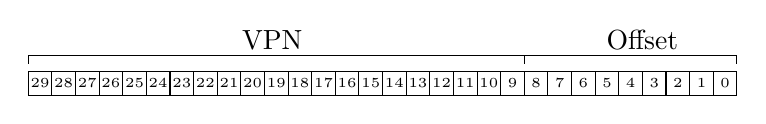
\begin{tikzpicture}
  % VPN
  \node at (3.1,0.7) (vpn){VPN};
  \draw (0, 0.4) -- (0,0.5);
  \draw (6.3, 0.4) -- (6.3,0.5);
  \draw (0, 0.5) -- (6.3,0.5);

  % Offset
  \node at (7.8,0.7) (off){Offset};
  \draw (6.3, 0.4) -- (6.3,0.5);
  \draw (9, 0.4) -- (9,0.5);
  \draw (6.3, 0.5) -- (9,0.5);

  \foreach \x [count=\xi from 0, evaluate=\xi as \num using int(29-\xi)] in
  {0,0.3,0.6,...,9}
  {
    \draw (\x, 0) rectangle (\x+0.3, 0.3);
    \node[font=\tiny] at (\x+0.15, 0.15) {\num};
  }
\end{tikzpicture}
\begin{itemize}
\item When chopping page table into pages, page table pages (PTP) usually have same \textbf{size} as virtual addr page: $S_{\text{VAP}} = S_{\text{PTP}} = 512$ bytes
\item Thus, each PTP will have $N_{\text{PTE}} = \frac{S_{\text{PTP}}}{S_{\text{PTE}}} = \frac{512}{4} = 128$ PTEs
\item To find each PTE, \texttt{PTIndex} need bits of $\log_2 N_{\text{PTE}} = \log_2 128 = 7$
\item The left 14 bits (30 - offset - \texttt{PTIndex}) used for Page Directory Index
\end{itemize}
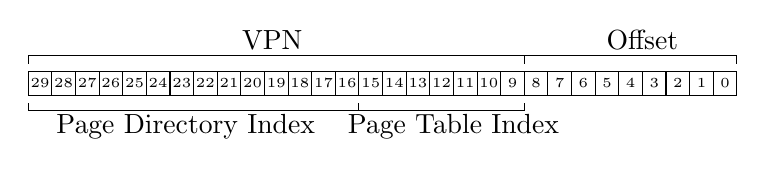
\begin{tikzpicture}
  % VPN
  \node at (3.1,0.7) (vpn){VPN};
  \draw (0, 0.4) -- (0,0.5);
  \draw (6.3, 0.4) -- (6.3,0.5);
  \draw (0, 0.5) -- (6.3,0.5);

  % Offset
  \node at (7.8,0.7) (off){Offset};
  \draw (6.3, 0.4) -- (6.3,0.5);
  \draw (9, 0.4) -- (9,0.5);
  \draw (6.3, 0.5) -- (9,0.5);

  \foreach \x [count=\xi from 0, evaluate=\xi as \num using int(29-\xi)] in
  {0,0.3,0.6,...,9}
  {
    \draw (\x, 0) rectangle (\x+0.3, 0.3);
    \node[font=\tiny] at (\x+0.15, 0.15) {\num};
  }

  % PDIndex
  \draw (0, -0.1) -- (0,-0.2);
  \draw (4.2, -0.1) -- (4.2,-0.2);
  \draw (0, -0.2) -- (4.2,-0.2);
  \node at (2,-0.4) (pdindex){Page Directory Index};

  % PTIndex
  \draw (4.2, -0.1) -- (4.2,-0.2);
  \draw (6.3, -0.1) -- (6.3,-0.2);
  \draw (4.2, -0.2) -- (6.3,-0.2);
  \node at (5.4,-0.4) (ptindex){Page Table Index};
\end{tikzpicture}
\begin{itemize}
\item this results in a \textbf{HUGE} PD itself: $2^{14}$ PEDs and requires 128 pages
\end{itemize}
\includegraphics[width=\linewidth]{imgs/huge_2level_pt}
\begin{itemize}
\item Splitting PD into 2 levels and each level has same bit width: 7
\item TLB miss causes additional memory accesses
\end{itemize}
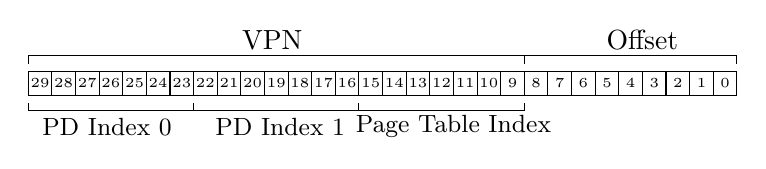
\begin{tikzpicture}
  % VPN
  \node at (3.1,0.7) (vpn){VPN};
  \draw (0, 0.4) -- (0,0.5);
  \draw (6.3, 0.4) -- (6.3,0.5);
  \draw (0, 0.5) -- (6.3,0.5);

  % Offset
  \node at (7.8,0.7) (off){Offset};
  \draw (6.3, 0.4) -- (6.3,0.5);
  \draw (9, 0.4) -- (9,0.5);
  \draw (6.3, 0.5) -- (9,0.5);

  \foreach \x [count=\xi from 0, evaluate=\xi as \num using int(29-\xi)] in
  {0,0.3,0.6,...,9}
  {
    \draw (\x, 0) rectangle (\x+0.3, 0.3);
    \node[font=\tiny] at (\x+0.15, 0.15) {\num};
  }

  % PDIndex 0
  \draw (0,   -0.1) -- (0,  -0.2);
  \draw (2.1, -0.1) -- (2.1,-0.2);
  \draw (0,   -0.2) -- (2.1,-0.2);
  \node at (1,-0.4) (pdindex0){\small PD Index 0};

  % PDIndex 1
  \draw (4.2, -0.1) -- (4.2,-0.2);
  \draw (2.1, -0.2) -- (4.2,-0.2);
  \node at (3.2,-0.4) (pdindex1){\small PD Index 1};

  % PTIndex 0
  \draw (4.2, -0.1) -- (4.2,-0.2);
  \draw (6.3, -0.1) -- (6.3,-0.2);
  \draw (4.2, -0.2) -- (6.3,-0.2);
  \node at (5.4,-0.4) (ptindex){\small Page Table Index};
\end{tikzpicture}

\includegraphics[width=\linewidth]{imgs/smaller_3level_pt}

\begin{itemize}
\item the bigger the page table, the faster a TLB miss can be serviced
\item memory-constrained (old) system, smaller page tables preferred
\end{itemize}

% \section*{Swapping (transparent to process)}
\begin{itemize}
\item For more than avail. physical memory $\to$ use 2nd storage, SSD etc.
\item Space on disk reserved to move pages back/forth to memory
\item OS reads/writes to swap space in \textbf{page-sized} units
\item OS needs to remember disk address of a given page
\item TLB uses this bit to track if a page is present in physical memory
\end{itemize}
\section*{Why hardware doesn't handle page faults}
\begin{enumerate}
\item page faults to disk are \emph{slow}; extra overheads of software are minimal
\item the hardware would have to understand swap space, how to issue I/Os to disk, and lots other details it currently doesn't know much about
\end{enumerate}
\section*{OS handles page faults via swapping}
while I/O is in flight, process will be in blocked state. Thus, OS will be free to run other ready processes while page fault is being serviced
\begin{enumerate}
\item page tables stores bits info about where to find the desired page
\item OS uses the bits in PTE for a disk address
\item On page fault, OS looks in PTE to find the address and issues request to disk to fetch page into memory
\item When disk I/O done, OS marks the page in PT as present, update PFN field of PTE to record in-memory location of newly-fetched page, and retry ix
\item This next attempt may cause TLB miss which would then be serviced and update TLB with addr translation (or update TLB directly)
\item a last restart would find the translation in TLB and proceed to fetch desired data/instruction from memory at translated physical address
\end{enumerate}
\section*{Page-Fault Control Flow Algorithm (Hardware)}
\begin{minipage}{.72\linewidth}
\begin{lstlisting}[language=c]
VPN = (VirtualAddress & VPN_MASK) >> SHIFT
(Success, TlbEntry) = TLB_Lookup(VPN)
if (Success == True) // TLB Hit
   if (CanAccess(TlbEntry.ProtectBits) == True)
      Offset = VirtualAddress & OFFSET_MASK
      PhysAddr = (TlbEntry.PFN << SHIFT) | Offset
      Register = AccessMemory(PhysAddr)
   else
      RaiseException(PROTECTION_FAULT)
else                 // TLB Miss
   PTEAddr = PTBR + (VPN * sizeof(PTE))
   PTE = AccessMemory(PTEAddr)
   if (PTE.Valid == False)
      RaiseException(SEGMENTATION_FAULT)
   else
      if (CanAccess(PTE.ProtectBits) == False)
         RaiseException(PROTECTION_FAULT)
      else if (PTE.Present == True)
         // assuming hardware-managed TLB
         TLB_Insert(VPN, PTE.PFN, PTE.ProtectBits)
         RetryInstruction()
      else if (PTE.Present == False)
         RaiseException(PAGE_FAULT)
\end{lstlisting}
\end{minipage}
\begin{minipage}{.28\linewidth}
  \includegraphics[width=\linewidth]{imgs/swap_cases}
\end{minipage}
\section*{Page-Fault Control Flow Algorithm (Software)}
\begin{minipage}{.72\linewidth}
\begin{lstlisting}[language=c]
PFN = FindFreePhysicalPage()
if (PFN == -1)                 // no free page found
    PFN = EvictPage()          // replacement algo
DiskRead(PTE.DiskAddr, PFN)  // sleep (wait for I/O)
PTE.present = True             // update page table:
PTE.PFN = PFN                  // present/translation
RetryInstruction()             // retry instruction
\end{lstlisting}
\end{minipage}
\begin{minipage}{.28\linewidth}
  \flushleft
  \begin{enumerate}
  \item check any free pages avail
  \item if not, ask bg thread to free
  \item when some pages avail, wake up orig thread
  \end{enumerate}
\end{minipage}

\begin{itemize}
\item when OS notices there're fewer than low watermark (LW) pages avail., a background thread responsible for freeing memory runs
\item bg thread evicts pages until there're high watermark (HW) pages avail.
\item bg swap/page daemon: disk efficiency $\uparrow$; work $\downarrow$, better idle time
\item OS groups pages and swaps them out at once $\to$ $\uparrow$ disk efficiency
\end{itemize}

% \columnbreak
% \section*{Swapping Policies (minimize cache miss/page fetch)}
\begin{itemize}
\item Average Memory Access Time (AMAT)=$T_{M}+(P_{\text{Miss}} + T_{D})$
\item $T_{M}$ the cost of accessing memory; $T_{D}$ the cost of accessing disk
\item $P_{\text{Miss}}$ the probability of not finding  data in cache (a miss) [0.0,1.0]
\item $P_{\text{Miss}} = 0.1$, $T_{D}=10$ms, $T_{M}$=100ns $\to$ AMAT = 1.0001ms
\item $P_{\text{Miss}} = 0.001$ ($P_{\text{Hit}} = 0.999$) $\to$ AMAT = 10.1$\mu$s (100 times faster)
\item In general, $P_{\text{Miss}} + P_{\text{Hit}} = 1.0$
\end{itemize}

\section*{Types of cache misses (3 categories)}
\begin{enumerate}
\item compulsory miss (aka cold-start miss): cache is empty (first reference)
\item capacity miss: no enough space $\to$ evict old to make room for new
\item conflict miss: arises due to (hardware) limits on where the item can be placed in cache.  Conflict miss doesn’t occur in the OS page cache, as the cache is
fully associative (a page can be placed anywhere)
\end{enumerate}

\section*{The optimal policy (by Belady), FIFO, Random, LRU, LFU}
\begin{itemize}
\item replace the page that will be accessed \textbf{furthest in the future}
\item Hard to implement (because hard to predict the future)
\item Useful as an ideal policy to compare with (can't do better than optimal)
\end{itemize}
\begin{itemize}
\item FIFO/Random: might evict important pages (to be ref-ed again soon)
\item \textbf{frequency} a page accessed frequently is perhaps important
\item \textbf{recency} a page accessed recently will perhaps be accessed again
\end{itemize}
\section*{Workload examples (100 unique pages)}
\begin{minipage}{0.33\linewidth}
  \includegraphics[width=\linewidth,height=3.5cm]{imgs/non_locality_workload}
\end{minipage}
\begin{minipage}{0.34\linewidth}
  \includegraphics[width=\linewidth,height=3.5cm]{imgs/eight_20_workload}
\end{minipage}
\begin{minipage}{0.33\linewidth}
  \includegraphics[width=\linewidth,height=3.5cm]{imgs/looping_workload}
\end{minipage}
\begin{minipage}{0.5\linewidth}
  \flushleft
  \begin{enumerate}
  \item no locality $\to$ any policy works
  \item when cache size $>$ workload, swap policy in use doesn't matter
  \item optimal performs better than other realistic policies
  \item for 80-20, LRU does better than random/FIFO
  \end{enumerate}
\end{minipage}
\begin{minipage}{0.5\linewidth}
  \flushleft
  \begin{enumerate}
  \item loops common in applications (eg databases)
  \item worst case scenario for FIFO and LRU
  \item A looping workload with N pages and cache size $<$ N pages always result in
0\% hit rate
  \end{enumerate}
\end{minipage}

\section*{Issues of implementing LRU}
\begin{itemize}
\item implementing history-based policies requires accounting of every memory ref $\to$ performance $\downarrow$ if not careful
\item possible hardware support: update time field in memory for each page
\item OS then scans time fields to find LRU page: expensive if page num $\uparrow$
\end{itemize}
\section*{Approximating LRU: clock algorithm}
\begin{itemize}
\item use a \textbf{use bit} (aka \textbf{reference bit} to page)
\item when page is accessed, set bit to 1 (done by hardware)
\item arrange all pages in a circular list and when replacement occurs
\item if use bit is 1, set it to 0 and move on; if use bit is 0, evict the page
\end{itemize}
\section*{Dirty Pages (regarding clock algorithm: whether a page is modified)}
\begin{itemize}
\item If page has been modified, do not evict (write to disk is expensive)
\item If page is clean, eviction is free (no need to write to disk)
\item hardware support should include a \textbf{dirty bit}
\end{itemize}
\section*{Belady's anomaly}
\begin{itemize}
\item In general, cache size $\uparrow \to$ cache hit rate $\uparrow$ but not true for FIFO
\item stack property: For algorithms (eg LRU) with this property, cache of size N + 1 naturally includes contents of a cache of size N
\item FIFO/Random (among others) do not obey the stack property; susceptible to anomalous behavior
\end{itemize}

% \section*{(most) Locks}
\begin{minipage}{.5\linewidth}
\begin{lstlisting}[language=c,xrightmargin=2pt]
// globally-allocated lock 'mutex'
lock_t mutex; // declare lock var
// ... other work ...
lock(&mutex);
balance = balance + 1;
unlock(&mutex);
\end{lstlisting}
\end{minipage}
\begin{minipage}{.5\linewidth}
  \begin{itemize}
  \item must declare a lock before using it
  \item lock available = unlocked, free $\to$ no thread holds it
  \item lock acquired = locked, held $\to$ exactly one thread holds it (likely in a critical section)
  \end{itemize}
\end{minipage}
\begin{itemize}
\item other info like which thread holds lock or a queue for ordering lock acquisition can be stored in lock but often hidden from user
\item calling \texttt{lock()} will try to acquire lock (1. free; 2. not free)
  \begin{enumerate}
  \item thread acquires lock and enters critical section; \textbf{owner} of lock
  \item thread waits (not return) and cannot enter critical section
  \end{enumerate}
\item calling \texttt{unlock()} will free the lock (1. no waiting thread; 2. opposite)
  \begin{enumerate}
  \item lock becomes free and any thread can try to acquire it
  \item one of waiting threads will acquire lock and enters critical section
  \end{enumerate}

\item \textbf{coarse-grained}: one big lock for access to critical section at any time
\item \textbf{fine-grained}: different locks to protect different data and data structs (allowing more threads in different locked code at once)
\end{itemize}
\section*{Evaluating Locks}
\begin{enumerate}
\item \textbf{correctness} lock provides \textbf{mutual exclusion}
\item \textbf{fairness} each thread gets a fair shot at acquiring the lock (once it's free); no thread contending for the lock starve while doing so
\item \textbf{performance} time overhead added by using the lock:
  \begin{enumerate}
  \item single thread (no contention) $\to$ what is the overhead?
  \item multiple threads contending for lock on single CPU
  \item lock perf. on multiple CPUs and threads contending for the lock
  \end{enumerate}
\end{enumerate}
\begin{minipage}{.5\linewidth}
\begin{lstlisting}[language=c,xrightmargin=2pt]
void lock() { // before entering
  DisableInterrupts();
}
void unlock() { // after leaving
  EnableInterrupts();
}
\end{lstlisting}
\end{minipage}
\begin{minipage}{.5\linewidth}
  \begin{itemize}
  \item one of earliest solution offers mutex by disabling interrupts
  \item code inside critical section (not interrupted) runs as if it were atomic
  \item invented for single-processor systems;  main advantage: simplicity
  \end{itemize}
\end{minipage}
\begin{enumerate}
\item \textbf{insecure} arbitrary thread will need to perform \emph{privileged} ops so greedy/malicious progs can monopolize CPU and exploit system
\item \textbf{importable} not working on multiprocessors: threads enter same critical section via other CPUs $\to$ null effect of disabling interrupts
\item \textbf{buggy} turning off interrupts for too long $\to$ lost useful/critical interrupts that make OS work as expected (e.g. disturb I/O awakening)
\end{enumerate}
Thus, limited use case: OS occasionally uses interrupt masking to guarantee atomicity when accessing its own data structures
\section*{Failed Attempt: Just Using Loads/Stores}
\begin{minipage}{.5\linewidth}
\begin{lstlisting}[language=c,xrightmargin=2pt]
typedef struct __lock_t
{ int flag; } lock_t;

void init(lock_t *mutex) {
  // 0: lock is avail | 1: held
  mutex->flag = 0; }

void lock(lock_t *mutex) {
  while (mutex->flag == 1) // TEST
     ; // spin-wait (do nothing)
  mutex->flag = 1; // now SET it }

void unlock(lock_t *mutex) {
   mutex->flag = 0; }
\end{lstlisting}
\end{minipage}
\begin{minipage}{.5\linewidth}
  \begin{itemize}
  \item use 1 var \texttt{flag} to indicate thread's ownership of lock
  \item when lock not free, other threads \textbf{spin-wait} in while loop
  \item once lock free, waiting thread gets lock $\to$ set flat to 1
  \item correctness problem: both of two threads can set flag to 1 (with interrupts) and enter same critical section $\to$ mutex \textbf{not} guaranteed
  \item performance issue: thread endless checks flag (spin-waiting) and wastes CPU cycles
  \end{itemize}
\end{minipage}
\section*{Working Spin Locks with Test-And-Set (atomic exchange)}
\begin{itemize}
\item test old value and simultaneously setting the mem location to new value
\item return the old value pointed by \texttt{old\_ptr} and set \texttt{new} at same time
\item this sequence of operations is performed \textbf{atomically}
\end{itemize}
\begin{minipage}{.7\linewidth}
\begin{lstlisting}[language=c]
int TestAndSet(int *old_ptr, int new) {
  int old = *old_ptr;// fetch old value at old_ptr
  *old_ptr = new;      // store new into old_ptr
  return old;          // return the old value
}

typedef struct __lock_t { int flag; } lock_t;

// 0: lock is avail, 1: lock is held
void init(lock_t *lock) { lock->flag = 0; }

void lock(lock_t *lock) {
   while (TestAndSet(&lock->flag, 1) == 1)
     ; // spin-wait (do nothing)
}

void unlock(lock_t *lock) { lock->flag = 0; }
\end{lstlisting}
\end{minipage}
\begin{minipage}{.3\linewidth}
  \flushleft
  \begin{itemize}
  \item make both \textbf{test} (old lock value) and \textbf{set} (new value) a single atomic op $\to$ only one thread acquires the lock $\to$ working mutual exclusion primitive
  \item On single CPU, needs a preemptive scheduler (interrupt via timer); otherwise a thread spins on a CPU and never gives it up
  \end{itemize}
\end{minipage}
\begin{enumerate}
\item \textbf{correctness} yes, only a single thread enters critical section at a time
\item \textbf{fairness} not generally, thread may spin forever $\to$ starve/zero fairness
\item \textbf{performance} \textbf{a} on single CPU, pretty bad: if N threads contending for the lock, each thread spins for duration of time slice before being timer-preempted. \textbf{b} on multiple CPU, reasonably well if \# of threads $\approx$ \# of CPUs and critical section is short (wasting fewer CPU cycles)
\end{enumerate}

\section*{Compare-and-Swap (SPARC) or Compare-and-Exchange (x86)}
\begin{minipage}{.65\linewidth}
\begin{lstlisting}[language=c]
// only diff with set-and-test shown below
int CompareAndSwap(int *ptr,
                     int expected, int new)
{
    int original = *ptr;
    if (original == expected)
       *ptr = new;
    return original;
}
void lock(lock_t *lock) {
   while(CompareAndSwap(&lock->flag,0,1) == 1)
      ; // spin
} // more powerful than test-and-set
\end{lstlisting}
\end{minipage}
\begin{minipage}{.35\linewidth}
  \flushleft
  \begin{itemize}
  \item test if value at addr \texttt{ptr} == expected;
  \item if so, update mem location \texttt{ptr} to new.
  \item If not, do nothing.
  \item In either case, return orig val at that mem location, thus allowing the code calling compare-and-swap to know if it succeeded
  \item for lock-free struct
  \end{itemize}
\end{minipage}
a simple spin lock built with it \texttt{==} test-and-set spin lock analyzed above
\section*{Load-Linked + Store-Conditional (MIPS, Alpha, PowerPC, ARM)}
\begin{minipage}{.65\linewidth}
\begin{lstlisting}[language=c]
int LoadLinked(int *ptr) { return *ptr; }
// atomic operation
int StoreConditional(int *ptr, int new) {
  if (no update to *ptr
      since LoadLinked to this address) {
     *ptr = new;
     return 1; // success!
  } else { return 0; }  // failed to update
}
// Using LL/SC To Build A Lock
void lock(lock_t *lock) {
  while (1) {
    while (LoadLinked(&lock->flag) == 1)
       ; // spin until it's zero
    if (StoreConditional(&lock->flag, 1) == 1)
       return;
      // if set-it-to-1 is a success: all done
      // otherwise: try it all over again
    }
}
void unlock(lock_t *lock) { lock->flag = 0; }
\end{lstlisting}
\end{minipage}
\begin{minipage}{.35\linewidth}
  \flushleft
  \begin{itemize}
  \item load-linked operation likes load ix $\to$ fetch a value from addr \texttt{ptr} and place in a register
  \item store-cond succeeds (and updates the val) \emph{only} if no intervening store to the addr has taken place
  \item if succeeded, returns 1; val at \texttt{ptr} $\to$ \texttt{new}
  \item if failed, returns 0; val at \texttt{ptr} \emph{not} updated
  \item suppose 2 threads both exec \texttt{LoadLinked} and proceed to store-cond
  \item at this point only 1 thread will succeed in updating flag to 1
  \end{itemize}
\end{minipage}
\begin{minipage}{.45\linewidth}
\begin{lstlisting}[language=c]
int FetchAndAdd(int *ptr) {
   int old = *ptr;
   *ptr = old + 1;
   return old; }
\end{lstlisting}
\end{minipage}
\begin{minipage}{.55\linewidth}
  \begin{itemize}
  \item atomically increments a val while returning old val at particular addr
  \item In Intel x86, implemented using the ADD instruction with a prefix LOCK
  \end{itemize}
\end{minipage}
\section*{Ticket lock using Fetch-and-Add (ensures progress for all threads)}
\begin{minipage}{.55\linewidth}
\begin{lstlisting}[language=c]
typedef struct __lock_t {
  int ticket;
  int turn;
} lock_t;
void lock_init(lock_t *lock) {
  lock->ticket = 0;
  lock->turn = 0;
}
void lock(lock_t *lock) {
  int myturn;
  myturn = FetchAndAdd(&lock->ticket);
  while (lock->turn != myturn)
     ; // spin
}
void unlock(lock_t *lock) {
   lock->turn = lock->turn + 1;
}
\end{lstlisting}
\end{minipage}
\begin{minipage}{.45\linewidth}
  \flushleft
  \begin{itemize}
  \item when a thread tries to acquire a lock, it first does an \textbf{atomic} fetch-and-add on the ticket
  \item that value is now this thread's ``turn'' (\texttt{myturn})
  \item then use globally shared \texttt{lock->turn} to determine which thread's turn
  \item a thread enters critical section if \texttt{myturn == turn}
  \item unlocking increments the turn so next waiting thread (if any) can enter critical section
  \item thread with ticket will be scheduled later on
  \end{itemize}
\end{minipage}
\section*{Yield (good with 2 threads but worse with more)}
\begin{minipage}{.5\linewidth}
\begin{lstlisting}[language=c]
void init() { flag = 0; }
void lock() {
  while (TestAndSet(&flag, 1) == 1)
    yield(); // give up the CPU
}
void unlock() { flag = 0; }
\end{lstlisting}
\end{minipage}
\begin{minipage}{.5\linewidth}
  \flushleft
  \begin{itemize}
  \item assume OS with \texttt{yeild()} (give up CPU and let others run)
  \item thread may be running, ready, or blocked; \texttt{yeild}: running $\to$ ready
  \item yielding thd \textbf{deschedules} itself
  \item works well with 2 thds (no spin)
  \end{itemize}
\end{minipage}
\begin{itemize}
\item suppose there are 100 threads contending for a lock repeatedly
\item if one thread acquires lock but gets preempted before releasing it, the other 99 will each call \texttt{lock()}, find lock held, and yield CPU
\item if RR sched, each of 99 run-and-yeild before lock-holder runs again
\item no 99 time slice spinning but cost of ctx switch is substantial (waste)
\item this approach does \emph{not} stress starvation: A thread may get
caught in endless yield loop while others repeatedly enter/exit critical section
\end{itemize}
\section*{Lock with queues (correct, reasonably fair, limited spinning)}
\begin{minipage}{.6\linewidth}
\begin{lstlisting}[language=c]
typedef struct __lock_t {
  int flag;
  int guard;
  queue_t *q;
} lock_t;
void lock_init(lock_t *m) {
  m->flag = 0;
  m->guard = 0;
  queue_init(m->q);
}
void lock(lock_t *m) {
  while (TestAndSet(&m->guard, 1) == 1)
     ; //acquire guard lock by spinning
  if (m->flag == 0) {
    m->flag = 1; // lock is acquired
    m->guard = 0;
  } else {
    queue_add(m->q, gettid());
+   setpark();  // avoid wakeup/waiting race
    m->guard = 0;
    park(); // syscall
  }
} // + indicates new code
void unlock(lock_t *m) {
  while (TestAndSet(&m->guard, 1) == 1)
     ; //acquire guard lock by spinning
  if (queue_empty(m->q))// no one wants it
    m->flag = 0;          // let go of lock
  else // hold lock for next thread
    unpark(queue_remove(m->q));
  m->guard = 0;
}
\end{lstlisting}
\end{minipage}
\begin{minipage}{.4\linewidth}
  \flushleft
  \begin{itemize}
  \item this approach doesn't avoid spin-waiting entirely: a spin-lock around \texttt{flag} and \texttt{queue} (lock is using)
  \item \texttt{guard} ensures queue is modified atomically
  \item waiting thread $\to$ queue and \texttt{park()} to sleep
  \item thread releasing lock $\to$ \texttt{unpark()} waiting threads
  \item time spent spinning is quite limited (just a few instructions inside lock and unlock code, instead of user-def critical section)
  \item if thread not acquired lock, adds itself to queue
  \item When a thread woken up, it is as if returning from \texttt{park()}; yet it does not hold \texttt{guard} at that point and thus cannot try to set \texttt{flag} to 1. lock passed directly from releasing-thd to next waiting thd. \texttt{flag} is not set to 0 in-between
  \item \texttt{setpark} makes \texttt{park} return immediately
  \end{itemize}
\end{minipage}

% \input{subs/ch29_locked_dt}
% \section*{Condition Variable (check a cond before continuing exec)}
\begin{minipage}{.58\linewidth}
\begin{lstlisting}[language=c]
volatile int done = 0;
void *child(void *arg) {
  printf("child\n");
  done = 1;
  return NULL;
}
int main(int argc, char *argv[]) {
  printf("parent: begin\n");
  pthread_t c;
  // create a child
  Pthread_create(&c, NULL, child, NULL);
  while (done == 0)
     ; // spin
  printf("parent: end\n");
  return 0;
}
\end{lstlisting}
\end{minipage}
\begin{minipage}{.42\linewidth}
  \flushleft
  \begin{itemize}
  \item expected output:
    \begin{itemize}
    \item[] \texttt{parent}: \texttt{begin}
    \item[] \texttt{child}
    \item[] \texttt{parent}: \texttt{end}
    \end{itemize}
  \item easy solution: spin on a cond var until it changes
  \item it works but \mo{very} \mo{inefficient}
  \item spinning wastes CPU cycles
  \item desired: put parent to sleep while waiting for child doing its work and then wake parent up to proceed
  \item need a condition variable as a more efficient checkpoint
  \end{itemize}
\end{minipage}
\begin{lstlisting}[language=c]
// referred to as wait() and signal() for simplicity hereafter
pthread_cond_wait(pthread_cond_t *c, pthread_mutex_t *m);
pthread_cond_signal(pthread_cond_t *c); // ^ take mutex as arg
\end{lstlisting}
\begin{lstlisting}[language=c]
int done = 0;
pthread_mutex_t m = PTHREAD_MUTEX_INITIALIZER;
pthread_cond_t c = PTHREAD_COND_INITIALIZER;
\end{lstlisting}
\begin{minipage}{.56\linewidth}
\begin{lstlisting}[language=c]
void thr_exit() {
  Pthread_mutex_lock(&m);
  done = 1;
  Pthread_cond_signal(&c);
  Pthread_mutex_unlock(&m);
}
void *child(void *arg) {
  printf("child\n");
  thr_exit();
  return NULL;
}
void thr_join() {
  Pthread_mutex_lock(&m);
  while (done == 0) // better than if
     Pthread_cond_wait(&c, &m);
  Pthread_mutex_unlock(&m);
}
int main(int argc, char *argv[]) {
  printf("parent: begin\n");
  pthread_t p;
  Pthread_create(&p, NULL, child, NULL);
  thr_join();
  printf("parent: end\n");
  return 0;
}
\end{lstlisting}
\end{minipage}
\begin{minipage}{.44\linewidth}
  \flushleft
  \begin{itemize}
  \item \texttt{wait()} puts calling thread to sleep and release the lock (done \mr{atomically})
  \item when sleeping thread wakes up (after some other thread signal), it must \mb{reacquire} lock before returning to caller
  \item thus preventing certain race conds when a thread is trying to put itself to sleep (while others contending for lock)
  \item suppose 1 CPU and 2 threads
  \end{itemize}
  \begin{enumerate}
  \item parent creates child and immediately calls \texttt{join()} to wait for child
  \item parent acquires lock, sees child not done $\to$ \texttt{wait()} (also release the lock)
  \item child grabs lock, runs, prints, then \texttt{exit()} to signal parent
  \item parent returns from \texttt{wait()}, reholds lock, unlocks, done
  \end{enumerate}
\end{minipage}
\begin{enumerate}
\item child runs immediately upon creation, sets \texttt{done} to 1, \texttt{signal()} to wake sleeping thread, but there is none, so child done and returns
\item parent runs \texttt{join()}, sees \texttt{done} is 1, so does \mr{not} wait and just returns
\end{enumerate}
\begin{minipage}{.5\linewidth}
\begin{lstlisting}[language=c,xrightmargin=2pt]
void thr_exit() {
  Pthread_mutex_lock(&m);
  Pthread_cond_signal(&c);
  Pthread_mutex_unlock(&m); }
void thr_join() {
  Pthread_mutex_lock(&m);
  Pthread_cond_wait(&c, &m);
  Pthread_mutex_unlock(&m); }
\end{lstlisting}
\end{minipage}
\begin{minipage}{.5\linewidth}
  \flushleft
  \begin{itemize}
  \item if no condition variable \texttt{done}
  \item child may run immediately and \texttt{exit()}, then \texttt{signal()} main
  \item but main has \mr{not} fallen asleep
  \item since child already \texttt{signal()} before and won't do that again, when main thread try to \texttt{wait()}, it waits forever $|$ [if no mutex $\downarrow$]
  \end{itemize}
\end{minipage}
\begin{minipage}{.5\linewidth}
\begin{lstlisting}[language=c,xrightmargin=2pt]
void thr_exit() { // signal first
 done = 1; // no one to wake up
 Pthread_cond_signal(&c); }
\end{lstlisting}
\end{minipage}
\begin{minipage}{.5\linewidth}
\begin{lstlisting}[language=c,xleftmargin=2pt]
void thr_join() { // wait later ->
 if (done == 0)    // sleep forever
   Pthread_cond_wait(&c); }
\end{lstlisting}
\end{minipage}
\section*{The Producer/Consumer (Bounded Buffer) Problem}
\begin{itemize}
\item buffer is shared by a single producer and a single consumer
\item consumer \mo{wait}s for item avail. in buffer before reading; producer \mo{wait}s buffer to be empty before writing: need mutex + cond var
\end{itemize}
\begin{minipage}{.5\linewidth}
\begin{lstlisting}[language=c,xleftmargin=0pt,xrightmargin=2pt,frame=lines]
int buffer; // single-item buffer
int count = 0; // init empty
// assume buffer empty
void put(int value) {
  assert(count == 0);
  count = 1;
  buffer = value;
} // broken `put', see below
int get() { // assume buffer full
  assert(count == 1);
  count = 0;
  return buffer;
} // broken `get', see below
\end{lstlisting}
\end{minipage}
\begin{minipage}{.5\linewidth}
\begin{lstlisting}[language=c,xleftmargin=2pt,xrightmargin=2pt,frame=lines]
int buffer[MAX]; int count = 0;
int fill_ptr = 0; int use_ptr = 0;
void put(int value) {
  buffer[fill_ptr] = value;
  fill_ptr = (fill_ptr + 1) % MAX;
  count++;
} // correct `put', see right ->
int get() {
  int tmp = buffer[use_ptr];
  use_ptr = (use_ptr + 1) % MAX;
  count--;
  return tmp;
} // correct `get', see right ->
\end{lstlisting}
\end{minipage}

\begin{minipage}{.63\linewidth}
\begin{lstlisting}[language=c,xleftmargin=0pt]
int loops;      // must init somewhere
cond_t cond;    // broken when two consumers
mutex_t mutex; // see text on the right
void *producer(void *arg) {
  int i;
  for (i = 0; i < loops; i++) {
    thread_mutex_lock(&mutex);              // p1
    if (count == 1)                         // p2
      Pthread_cond_wait(&cond, &mutex); // p3
    put(i);                                 // p4
    Pthread_cond_signal(&cond);             // p5
    Pthread_mutex_unlock(&mutex);           // p6
  }
}
void *consumer(void *arg) {
  int i;
  for (i = 0; i < loops; i++) {
    Pthread_mutex_lock(&mutex);             // c1
    if (count == 0)                         // c2
      Pthread_cond_wait(&cond, &mutex); // c3
    int tmp = get();                        // c4
    Pthread_cond_signal(&cond);             // c5
    Pthread_mutex_unlock(&mutex);           // c6
    printf("%d\n", tmp);
  }
}
\end{lstlisting}
\end{minipage}
\begin{minipage}{.4\linewidth}
  \flushleft
  \begin{itemize}
  \item works well \mo{only} for single producer/consumer
  \item if with $p_1$ and $c_1$, $c_2$:
  \item $c_1$ runs first, acquires lock \mb{c1}, checks buf \mb{c2}, which is empty, so it releases lock and waits \mb{c3} (go to sleep)
  \item $p_1$ runs, acquires lock \mb{p1}, checks \mb{p2} and fills buf \mb{p4}, wakes up $c_1$ \mb{p5} (buf full). $p_1$ goes to sleep \mb{p6}, \mb{p1}-\mb{p3}
  \item $c_2$ runs (before $c_1$ has a chance) and consumes existing item \mb{c1}-\mb{c2}, \mb{c4}-\mb{c6}, skipping \mb{c3} due to buf full
  \item $c_1$ resumes, acquires lock, attempts to \texttt{get()} [\mb{c4}], \mr{without re-checking} \texttt{count}, as check was done before it went to sleep \mb{c2}
  \item Signaling only wakes up thread; it is a \mr{hint} that state
of world has changed
  \end{itemize}
\end{minipage}
\begin{minipage}{.64\linewidth}
\begin{lstlisting}[language=c,xleftmargin=0pt]
void *producer(void *arg) {
  int i;
  for (i = 0; i < loops; i++) {
    thread_mutex_lock(&mutex);              // p1
-   if (count == 1)                         // p2
+   while (count == 1)                      // p2
      Pthread_cond_wait(&cond, &mutex); // p3
    put(i);                                 // p4
void *consumer(void *arg) {
  int i;
  for (i = 0; i < loops; i++) {
    Pthread_mutex_lock(&mutex);             // c1
-   if (count == 1)                         // c2
+   while (count == 0)                      // c2
      Pthread_cond_wait(&cond, &mutex); // c3
    int tmp = get();                        // c4
\end{lstlisting}
\end{minipage}
\begin{minipage}{.4\linewidth}
  \flushleft
  \begin{itemize}
  \item fix: change \texttt{if} to \texttt{while}
  \item when $c_1$ wakes up, it \mo{recheck}s \texttt{cond} \mb{c2}; if buf empty, $c_1$ sleeps (\mb{c3})
  \item there is \mr{still one bug}:
  \item $c_1$, $c_2$ runs first and both go to sleep (\mb{c3})
  \item $p_1$ runs, fills buf, wakes $c_1$, loops back (\mb{p1}-\mb{p6}), waits on same cond (buf full $\to$ go to sleep, \mb{p2}-\mb{p3})
  \item $c_1$ wakes, returns from \texttt{wait()} \mb{c3}, re-checks \mb{c2}, takes val \mb{c4} (continued ...)
  \end{itemize}
\end{minipage}
\vspace{-.8em}
\begin{itemize}
\item if $c_1$ wakes $c_2$ (\mb{c5}), $c_2$ finds buf empty (\mb{c2}) and goes back to sleep (\mb{c3})
\item since no \mb{c5} from $c_2$, $p_1$ keeps sleeping, $c_1$ falls asleep \mb{c1}-\mb{c3}; all sleeping...
\item Signaling must be more directed: consumer should wake only producers
\item producers wait on cond \texttt{empty} and signal \texttt{fill}; consumers wait on \texttt{fill} and signal \texttt{emtpy}
\item a consumer never accidentally wakes a consumer and vice versa
\end{itemize}
\begin{minipage}{.55\linewidth}
\begin{lstlisting}[language=c,xleftmargin=-1em,xrightmargin=-4pt,frame=lines]
cond_t empty, fill; mutex_t mutex;
void *producer(void *arg) {
  int i;
  for (i = 0; i < loops; i++) {
    thread_mutex_lock(&mutex);
    while (count == 1)
     Pthread_cond_wait(&empty,&mutex);
    put(i);
    Pthread_cond_signal(&fill);
    Pthread_mutex_unlock(&mutex);
  }
}
\end{lstlisting}
\end{minipage}
\begin{minipage}{.55\linewidth}
\begin{lstlisting}[language=c,xleftmargin=-2.8em,frame=lines]
void *consumer(void *arg) {
  int i;
  for (i = 0; i < loops; i++) {
    Pthread_mutex_lock(&mutex);
    if (count == 0)
      Pthread_cond_wait(&fill,&mutex);
    int tmp = get();
    Pthread_cond_signal(&empty);
    Pthread_mutex_unlock(&mutex);
    printf("%d\n", tmp);
  }
}
\end{lstlisting}
\end{minipage}
\section*{Covering Conds (covers all cases where a thread needs to wake up)}
\begin{itemize}
\item \texttt{wait()} and \texttt{signal()} approach to thread synchronization assumes the waiting condition is the \textbf{same} for all threads
\item When multiple waiting threads have different conditions: a multi-thread memory allocator $\to$ When a thread frees memory, it should signal which thread to indicate more memory is available?
\end{itemize}
\begin{minipage}{.6\linewidth}
\begin{lstlisting}[language=c,xleftmargin=4pt]
// how many bytes of the heap are free
int bytesLeft = MAX_HEAP_SIZE;
// need lock and condition
cond_t c;  mutex_t m;
void *allocate(int size) {
  Pthread_mutex_lock(&m);
  while (bytesLeft < size)
    Pthread_cond_wait(&c, &m);
  void *ptr = ...; // get mem from heap
  bytesLeft -= size;
  Pthread_mutex_unlock(&m);
  return ptr;
}
void free(void *ptr, int size) {
  Pthread_mutex_lock(&m);
  bytesLeft += size;
- Pthread_cond_signal(&c);// signal whom?
+ Pthread_cond_broadcast(&c);
  Pthread_mutex_unlock(&m);
 }
\end{lstlisting}
\end{minipage}
\begin{minipage}{.4\linewidth}
  \flushleft
  \begin{itemize}
  \item assume 0 bytes free now
  \item $T_a$ calls \texttt{allocate(100)}
  \item $T_b$ calls \texttt{allocate(10)}
  \item Both $T_a$ and $T_b$ wait on cond and go to sleep due to no enough free bytes to satisfy either of requests
  \item $T_c$ calls \texttt{free(50)} and try to signal a thread
  \item it might wake $T_a$ instead of $T_b$ (suitable in this case)
  \item $T_a$ remains waiting and code not working
  \item Lampson and Redell suggest to wake up \mb{all} waiting threads by \texttt{phthread\_cond\_broadcast()}
  \end{itemize}
\end{minipage}
The downside is a negative performance impact: needlessly wake up many waiting threads that shouldn't (yet) be awake. Those threads will simply wake up, re-check cond, and then go immediately back to sleep
\begin{tcolorbox}[left=0mm, top=1mm, right=0mm, rightlower=0mm, bottom=1mm,
  title=Always hold the lock while signaling,halign title=center]
There are some cases where it is likely OK not to, but probably is something you should avoid. Thus, for simplicity, \textbf{hold the lock when calling signal}. The converse of this tip -- hold lock when calling wait -- is \textbf{mandated} by the semantics of wait: wait always
(a) assumes lock is held when calling it, (b) releases said lock when
putting caller to sleep, and (c) re-acquires lock just before returning. Thus, the generalization is correct:\textbf{ hold the lock when calling signal or wait}, and you will always be in good shape.
\end{tcolorbox}
\begin{tcolorbox}[left=0mm, top=1mm, right=0mm, rightlower=0mm, bottom=1mm,
  title=Use \texttt{while} (not \texttt{if}) for conditions,
  halign title=center]
When checking for a condition in a multi-threaded program, using a
\texttt{while} loop is always correct; using an if statement only might be, depending on what signaling does. Using while loops around conditional checks also handles the case where \textbf{spurious wakeups} occur. In some thread packages, due to implementation details, it's possible that 2 threads get woken up though a single signal. Spurious wakeups are further reason to re-check the condition a thread is waiting on.
\end{tcolorbox}

% \input{subs/ch31_sem}
% \section*{Atomicity-Violation Bugs (Non-Deadlock)}
\begin{minipage}{0.5\linewidth}
\begin{lstlisting}[language=c]
Thread 1::
if (thd->proc_info) {
  fputs(thd->proc_info, ...);
}       // ^ may deref NULL
Thread 2::
thd->proc_info = NULL;
\end{lstlisting}
\end{minipage}
\begin{minipage}{0.5\linewidth}
  \flushleft
  \begin{itemize}
  \item two $T$s access \texttt{proc\_info} in \texttt{thd}
  \item if $T_1$ checked but interrupted by $T_2$ before calling \texttt{fputs}
  \item $T_2$ sets pointer to \texttt{NULL}
  \item $T_1$ resumes and deref \texttt{NULL} ptr, BOM!
  \end{itemize}
\end{minipage}
\begin{itemize}
\item the code has an atomicity assumption about the check for non-NULL of \texttt{proc\_info} and the usage of \texttt{proc\_info} in the \texttt{fputs()} call
\item when the assumption is incorrect, the code will not work as desired
\end{itemize}
\begin{lstlisting}[language=c]
pthread_mutex_t pinfo_lock = PTHREAD_MUTEX_INITIALIZER;
\end{lstlisting}
\begin{minipage}{0.5\linewidth}
\begin{lstlisting}[language=c]
Thread 1::
pthread_mutex_lock(&pinfo_lock);
if (thd->proc_info) {
   fputs(thd->proc_info, ...);
}
pthread_mutex_unlock(&pinfo_lock);
\end{lstlisting}
\end{minipage}
\begin{minipage}{0.5\linewidth}
\begin{lstlisting}[language=c,xleftmargin=4pt]
// lock the critical section
Thread 2::
pthread_mutex_lock(&pinfo_lock);
thd->proc_info = NULL;
pthread_mutex_unlock(&pinfo_lock);
thd->proc_info = NULL;
\end{lstlisting}
\end{minipage}
\section*{Order-Violation Bugs (Non-Deadlock)}
\begin{minipage}{0.5\linewidth}
\begin{lstlisting}[language=c]
Thread 1::
void init() {
 mThread = PR_CreateThd(mMain,...);
}
\end{lstlisting}
\end{minipage}
\begin{minipage}{0.5\linewidth}
\begin{lstlisting}[language=c,xleftmargin=4pt]
Thread 2::
void mMain(...) {
  mState = mThread->State;
}// may deref NULL ^
\end{lstlisting}
\end{minipage}
\begin{itemize}
\item $T_2$ assumes \texttt{mThread} already init (non-NULL) while accessing it
\item yet if $T_2$ runs before $T_1$ $\to$ \texttt{mThread == NULL}, BOM! deref NULL ptr
\item to fix this type of bug $\to$ use \mo{cond var}/\mo{semaphore} to enforce ordering
\end{itemize}
\begin{lstlisting}[language=c]
pthread_mutex_t mtLock = PTHREAD_MUTEX_INITIALIZER; // lock
pthread_cond_t  mtCond = PTHREAD_COND_INITIALIZER;  // cond var
int mtInit = 0; // state variable
Thread 1::
void init() {
  // other work ...
  mThread = PR_CreateThread(mMain, ...);
  // signal that the thread has been created...
  pthread_mutex_lock(&mtLock);
  mtInit = 1; // set state
  pthread_cond_signal(&mtCond);
  pthread_mutex_unlock(&mtLock);
  // other work ...
}
Thread 2::
void mMain(...) {
  // other work ...
  // wait for the thread to be initialized...
  pthread_mutex_lock(&mtLock);
  while (mtInit == 0)
    pthread_cond_wait(&mtCond, &mtLock); // wait for state to be set
  pthread_mutex_unlock(&mtLock);
  mState = mThread->State;
  // other work ...
}
\end{lstlisting}
\begin{minipage}{0.5\linewidth}
  \section*{Deadlock}
\begin{lstlisting}[language=c,frame=lines]
Thread 1::
pthread_mutex_lock(L1);
pthread_mutex_lock(L2);
Thread 2::
pthread_mutex_lock(L1);
pthread_mutex_lock(L2);
\end{lstlisting}
  \flushleft
  \begin{itemize}
  \item deadlock \emph{may} occur when
  \item $T_1$ holds \texttt{L1}, waiting for \texttt{L2}
  \item $T_2$ holds \texttt{L2}, waiting for \texttt{L1}
  \end{itemize}
\end{minipage}
\begin{minipage}{0.5\linewidth}
  \includegraphics[width=\linewidth,height=3.6cm]{imgs/deadlocks1}
\end{minipage}
\section*{Reasons for Deadlock}
\begin{enumerate}
\item circular dependencies between threads and resources, such that none of the threads can acquire the required resources to make progress
\item encapsulation: modularity does not mesh well with locking
\end{enumerate}
\section*{4 must-hold conds for a deadlock to occur (any unmet, no deadlock)}
\begin{itemize}
\item \textbf{Mutual exclusion} Threads claim exclusive control of resources that they require (e.g. a thread grabs a lock)
\item \textbf{Hold-and-wait} Threads hold resources they already acquired (e.g. locks) while waiting for extra resources (locks they wish to acquire)
\item \textbf{No preemption} can't forcibly rm resources from $T$s holding them
\item \textbf{Circular wait} a circular chain of $T$s such that each $T$ holds one or more resources (e.g. locks) being requested by the next $T$ in the chain
\end{itemize}
\section*{Prevent circular wait $\to$ total/partial ordering on lock acquisition}
\begin{itemize}
\item if \emph{only} 2 locks (\texttt{L1},\texttt{L2}), strict ordering: always acquire \texttt{L1} before \texttt{L2}
\item lock acquisition must respect the partial ordering (reflexive, transitive, anti-symmetric) $\to$ guarantee no circularity
\end{itemize}
\begin{minipage}{0.5\linewidth}
\begin{lstlisting}[language=c,xleftmargin=2pt]
// fn need to grabs two locks
do sth(mutex t *m1, mutex t *m2)
\end{lstlisting}
  \begin{itemize}
  \item if always grabs \texttt{m1} before \texttt{m2} (or \texttt{m2} before \texttt{m1}) $\to$ may deadlock
  \item $\because T_1$ calls \texttt{do\_sth(m1, m2)} while $T_2$ calls \texttt{do\_sth(m2, m1)} $\to$ deadlock
  \item $T_1$ waits for \texttt{m2}; $T_2$ waits for \texttt{m1}
  \item fix: enforce ordering by lock addr
  \end{itemize}
\end{minipage}
\begin{minipage}{0.5\linewidth}
\begin{lstlisting}[language=c,xleftmargin=4pt,framextopmargin=1pt]
// grab in high-to-low addr order
if (m1 > m2) {
  pthread_mutex_lock(m1);
  pthread_mutex_lock(m2);
} else {
  pthread_mutex_lock(m2);
  pthread_mutex_lock(m1);
}
// assume m1 != m2 (not same lock)
\end{lstlisting}
\end{minipage}
\section*{Prevent hold-and-wait $\to$ acquire all locks at once, atomically}
\begin{minipage}{0.75\linewidth}
\begin{lstlisting}[language=c,xleftmargin=2pt]
pthread_mutex_lock(prevention); // begin acquisition
pthread_mutex_lock(L1);
pthread_mutex_lock(L2);
...
pthread_mutex_unlock(prevention); // end
\end{lstlisting}
\end{minipage}
\begin{minipage}{0.3\linewidth}
  \flushleft
  \begin{itemize}
  \item \mb{must} first grab \texttt{prevention} lock
  \item ensure no untimely $T$ switch can occurs $\to$ avoid deadlock
  \end{itemize}
\end{minipage}
\begin{itemize}
\item Ok for $T$ to acquire \texttt{L1}$\cdots$\texttt{L2} in any order $\because$ it already holding \texttt{L}$_\text{prevention}$
\item must know exactly which locks must be held and acquire ahead of time
\item concurrency $\downarrow$ $\because$ must acquire all locks at once even when not need to
\end{itemize}
\begin{minipage}{0.56\linewidth}
\section*{Add Preemption: imperfect, working}
\begin{lstlisting}[language=c,xleftmargin=2pt]
top:
  pthread_mutex_lock(L1);
  if (pthread_mutex_trylock(L2) != 0) {
    pthread_mutex_unlock(L1);
    goto top;
  }
\end{lstlisting}
\end{minipage}
\begin{minipage}{0.44\linewidth}
  \flushleft
  \begin{itemize}
  \item deadlock-free, ordering-robust lock acquisition protocol:
  \item try to grab lock if available $\to$ success
  \item if lock held by other $\to$ error; try again later
  \end{itemize}
\end{minipage}
\begin{itemize}
\item $T_{\text{other}}$ could follow same protocol but grab lock in order of \texttt{L2} then \texttt{L1}
\item this leads to \mo{livelock}: both systems running through this code sequence repeatedly (thus not a deadlock), but progress not being made
\item add a random delay before looping back and trying over again $\to$ decreasing the odds of repeated interference among competing threads
\item[1.] if \texttt{L1} gets dropped in some routine, go-back $\to$ more complex
\item[2.] if along \texttt{L1}, extra mem also acquired, must ensure to release mem too
\item[3.] \emph{not} really \emph{add} preemption, but just preempt its own lock ownership
\end{itemize}
\section*{Prevent Mutual Exclusion (lock-free data struct + hardware help)}
\begin{minipage}{0.5\linewidth}
\begin{lstlisting}[language=c]
int CompAndSwap(
  int *addr, int expected, int new
) {
  if (*addr == expected) {
    *addr = new;
    return 1; // success
  }
  return 0; // failure
} // atomic ix provided by hardware
\end{lstlisting}
\end{minipage}
\begin{minipage}{0.5\linewidth}
\begin{lstlisting}[language=c,xleftmargin=2pt]
void AtomicIncrement(
  int *val, int amt
) {
  do {
    int old = *val;
  } while (
  CompAndSwap(val, old, old + amt)
  == 0); // if val == old, inc old
} // else keep trying
\end{lstlisting}
\end{minipage}
livelock still possible; robust solution will be more complex than above\newline
\begin{minipage}{0.55\linewidth}
\section*{list insertion example}
\begin{lstlisting}[language=c,frame=none,xleftmargin=-6pt]
// thread-unsafe: race condition
void insert(int value) {
  node_t *n = malloc(sizeof(node_t));
  assert(n != NULL);
  n->value = value;
  n->next = head;
  head = n;
}
\end{lstlisting}
\end{minipage}
\begin{minipage}{0.5\linewidth}
\begin{lstlisting}[language=c,frame=none,xleftmargin=-18pt]
void insert(int value) {
  node_t *n = malloc(sizeof(node_t));
  assert(n != NULL);
  n->value = value;
  pthread_mutex_lock(listlock);
  n->next = head;
  head = n;
  pthread_mutex_unlock(listlock);
} // lock critical section
\end{lstlisting}
\end{minipage}
\begin{minipage}{0.68\linewidth}
\begin{lstlisting}[language=c]
void insert(int value) {
  node_t *n = malloc(sizeof(node_t));
  assert(n != NULL);
  n->value = value;
  do {
    n->next = head;
  } while (CompAndSwap(&head, n->next, n) == 0);
} // retry again with new head by other thread
\end{lstlisting}
\end{minipage}
\begin{minipage}{.32\linewidth}
  \flushleft
  \begin{itemize}
  \item point \texttt{next} to curr head and try to make the node new head
  \item this will fail if some other $T$ successfully swapped in a new head in meanwhile
  \item then try again
  \end{itemize}
\end{minipage}
\section*{Deadlock Avoidance via Scheduling}
\begin{minipage}{.4\linewidth}
  \begin{tabular}[ht]{lllll}
    Lock        & \texttt{T1} & \texttt{T2} & \texttt{T3} & \texttt{T4} \\
    \texttt{L1} & yes & yes & \mr{no} & no \\
    \texttt{L2} & yes & yes & yes & no \\
  \end{tabular}
\end{minipage}
\begin{minipage}{.6\linewidth}
  \includegraphics[width=.9\linewidth,height=1.8cm]{imgs/threadsdeadlock2}
\end{minipage}
\begin{itemize}
\item A smart scheduler could ensure T1 and T2 are not run at the same time $\to$ no deadlock could ever arise
\item  it is OK for (T3 and T1) or (T3 and T2) to overlap. Even
though T3 grabs lock \texttt{L2}, it can never cause a deadlock by running concurrently with other threads because it only grabs one lock
\end{itemize}
\begin{minipage}{.4\linewidth}
  \begin{tabular}[ht]{lllll}
    Lock        & \texttt{T1} & \texttt{T2} & \texttt{T3} & \texttt{T4} \\
    \texttt{L1} & yes & yes & \mr{yes} & no \\
    \texttt{L2} & yes & yes & yes & no \\
  \end{tabular}
\end{minipage}
\begin{minipage}{.6\linewidth}
  \includegraphics[width=\linewidth,height=1.8cm]{imgs/threadsdeadlock3}
\end{minipage}
\begin{itemize}
\item T1, T2, and T3 all need to grab both locks \texttt{L1} and \texttt{L2} at some point
\item static scheduling leads to conservative approach: T1, T2, T3 all run on same processor: $\to T_{\text{total-completion-time}} \uparrow$ considerably
\item deadlock avoidance: not a widely-used general-purpose solution
\end{itemize}
\section*{Detect and Recover}
\begin{itemize}
\item allow deadlocks to occasionally occur $\to$ reboot once detected it
\item this non-solution is indeed pragmatic if deadlocks are rare
\item Many DBMS employ deadlock detection and recovery techniques
\item deadlock detector runs periodically, building a resource graph and checking for cycles; when there's a cycle (deadlock), sys needs reboot
\end{itemize}
\begin{tcolorbox}[left=0mm, top=1mm, right=0mm, rightlower=0mm, bottom=1mm,
  title=USE ATOMIC OPERATIONS,
  halign title=center]
  The idea behind making a series of actions \textbf{atomic}: ``all or nothing''. It should either appear as if all of the actions you wish to group together occurred, or that none of them occurred, with no in-between state visible. Sometimes, the grouping of many actions into a single atomic action is called a \textbf{transaction}
\end{tcolorbox}
\begin{tcolorbox}[left=0mm, top=1mm, right=0mm, rightlower=0mm, bottom=1mm,
  title= DON'T ALWAYS DO IT PERFECTLY (TOM WEST'S LAW),
  halign title=center]
  ``Not everything worth doing is worth doing well'': If a bad thing happens rarely, certainly one should not spend much effort to prevent it, \emph{particularly if} the cost of the bad things is small. With pressing deadlines and other real-world concerns, one will always have to decide which aspects of a system to build well and which to put aside
\end{tcolorbox}

\section*{I/O Devices (allows information to persist; RAM is volatile)}
\begin{minipage}{.5\linewidth}
\includegraphics[width=\linewidth]{imgs/prototypical_sys_arch}
\end{minipage}
\begin{minipage}{.5\linewidth}
\includegraphics[width=\linewidth]{imgs/modern_sys_arch}
\end{minipage}
\begin{minipage}{.5\linewidth}
  \flushleft
  \begin{itemize}
  \item The faster a bus is, the shorter it must be $\to$ high-performance memory bus doesn't have much room for many devices
  \item components that demand high performance (such as graphics card) placed nearer CPU
  \item lower performance components are further away
  \end{itemize}
\end{minipage}
\begin{minipage}{.5\linewidth}
  \flushleft
  \begin{itemize}
  \item modern sys use specialized chipsets and faster point-to-point inter-conn to $\uparrow$ performance; USB (Universal Serial Bus) is used for low performance devices
  \item OS handles device management (and access); OS exposes uniform interface to applications
  \item IO is interrupt driven
  \end{itemize}
\end{minipage}
\begin{minipage}{.65\linewidth}
\includegraphics[width=\linewidth]{imgs/otherio}
\end{minipage}
\begin{minipage}{.35\linewidth}
  \flushleft
  \begin{itemize}
  \item Northbridge, aka memory controller hub
  \item Southbrigge, aka I/O Controller Hub (Intel) or Fusion Controller Hub (AMD)
  \item southbridge connected to CPU through northbridge which has a direct connection
  \end{itemize}
\end{minipage}
\section*{Canonical Devices (an abstraction with 2 components)}
\includegraphics[width=\linewidth]{imgs/canonical_dev}
\begin{itemize}
\item \textbf{status} register to be read to see the current status of the device
\item \textbf{command} register to tell the device to perform a certain task
\item \textbf{data} register pass data to the device, or get data from
the device
\end{itemize}
\begin{enumerate}
\item \textbf{hardware interface} presents to the rest of the system. Hardware must present some kind of interface that allows the system
software to control its operation. Thus, all devices have some specified
interface and protocol for typical interaction
\item \textbf{internal structure}, implementation specific and responsible for implementing the abstraction the device presents to the system
  \begin{itemize}
  \item Very simple devices will have one/a few hardware chips
  \item more complex devices will include a simple CPU, some general purpose
memory, and other device-specific chips, e.g modern RAID controllers might consist of hundreds of thousands of lines of firmware (i.e. software within a hardware device)  to impl. its functionality
  \end{itemize}
\end{enumerate}
\section*{Canonical Protocol (4 steps, simple yet inefficient)}
\begin{enumerate}
\item OS waits until the device ready to receive a command by repeatedly reading the status register (\textbf{polling} the device)
\item OS sends some data down to data register
  \begin{itemize}
  \item multiple writes to transfer a disk block (say 4KB) to the device
  \item if main CPU involved (as in this case) $\to$ \textbf{programmed I/O} (PIO)
  \end{itemize}
\item OS writes a command to command register $\to$ implicitly tell the device that data is present and device should begin working on the command
\item OS waits for the device to finish by again polling it in a loop, waiting to see if it is finished (return code for success/error)
\end{enumerate}
\begin{lstlisting}[language=c]
While (STATUS == BUSY)
    ; // wait until device is not busy
Write data to DATA register // set up everything before any cmd exec
Write command to COMMAND register
    (starts the device and executes the command)
While (STATUS == BUSY)
    ; // wait until device is done with your request
\end{lstlisting}
\section*{Lowering CPU Overhead with Interrupts}
\begin{minipage}{.5\linewidth}
\includegraphics[width=\linewidth]{imgs/iopolling}
\end{minipage}
\begin{minipage}{.5\linewidth}
\includegraphics[width=\linewidth]{imgs/iointerrupt}
\end{minipage}
\begin{minipage}{.5\linewidth}
  \flushleft
  \begin{enumerate}
  \item $P_1$ runs on CPU for some time (repeated \texttt{1} on CPU line)
  \item then issues I/O request to disk to read some data
  \item OS spins, polling status of device repeatedly until I/O completes
  \item disk serves req; $P_1$ can run again
  \end{enumerate}
\end{minipage}
\begin{minipage}{.5\linewidth}
  \flushleft
  \begin{enumerate}
  \item OS runs $P_2$ on CPU while disk services $P_1$'s request
  \item When disk request is done, an interrupt occurs
  \item OS wakes up $P_1$, runs it again
  \item \mb{both} CPU and disk get properly utilized during the middle
  \end{enumerate}
\end{minipage}
\begin{tcolorbox}[left=0mm, top=1mm, right=0mm, rightlower=0mm, bottom=1mm,
  title= Interrupts \mr{NOT always} better than polling,
  halign title=center]
  Although interrupts allow for overlap of computation and I/O, they only
  really \mb{make sense for slow devices}. Otherwise, the cost of interrupt handling and context switching may outweigh the benefits interrupts provide.  If a device performs its tasks \emph{very quickly}: the 1st poll usually finds the device done with task. Using an interrupt in this case will actually \emph{slow down} the system: switching to another process, handling the interrupt, and switching back to the issuing process is expensive.

  There are also cases where a flood of interrupts may overload a system and lead it to \textbf{livelock}; in such cases, polling provides more control to the OS in its scheduling and thus is again useful.
\end{tcolorbox}
\begin{itemize}
\item if a device is fast, best to poll; if it's slow, best to interrupt (overlap)
\item If device speed is unknown (sometimes fast, sometimes slow), best to \textbf{hybrid}: polls for a short while and if device not yet finished, interrupts
\item This \textbf{two-phased} approach may achieve the best of both worlds
\end{itemize}
In networks, when a huge stream of incoming packets each generate an interrupt, OS may \textbf{livelock}: find itself only processing interrupts and never running a user-level process and actually servicing requests
\begin{itemize}
\item a web server with a load burst $\because$ it became top-ranked on hacker news
\item In this case, it's better to occasionally poll to better control what's happening in system and allow server to fulfill some requests before going back to the device to check for more packet arrivals
\end{itemize}
Another interrupt-based optimization is \textbf{coalescing}:
\begin{itemize}
\item a device first waits for a bit before delivering its interrupt to CPU
\item While waiting, other requests may soon complete $\to$ multiple interrupts can be coalesced into a single delivery $\to$ lowering overhead
\item yet waiting too long $\to$ request latency $\uparrow$: common trade-off in systems
\end{itemize}
\section*{More Efficient Data Movement With DMA}
\end{multicols*}
\end{document}
